\section{A unified operational continuum limit}
\label{sec:unified-operational-continuum}

\textbf{Status: \StatusAbstract\ for the joint-interface theorem;
\StatusNumerical\ for its FLRW and four-dimensional tensor realization;
\StatusOpen\ for autonomous selection of the continuum phase, the
Einstein--Hilbert action, and a universal Newton coefficient.}

The order--volume and same-update results close two different interfaces.
The first reconstructs a Lorentzian metric--measure geometry from certified
response order and additive record capacity.  The second compares a Ramsey
response with the Euler derivative of one declared finite action.  Neither
statement alone proves that the geometry in the field equation is the one
reconstructed from the microscopic records.  Two separately convergent
sequences can approach inequivalent metrics, or can silently use different
refinement maps and actions.

The companion work \cite{XuUnifiedContinuum2026} closes this compatibility
problem for one explicit refinement family.  Its main requirement is
stronger than simultaneous convergence but weaker than autonomous action
selection: the order, capacity, and phase branches are evaluated
independently, while all three consume the same finite registers and the
same lattice spacing.

\subsection{One update record and two independent pipelines}

Let \(h\downarrow0\) label finite event sets \(X_h\).  A refinement record is
\begin{equation}
 {\cal R}_h=(X_h,q_h,\kappa_h,K_h,\Gamma_h,{\cal I}_h),
 \label{eq:unified-record}
\end{equation}
where \(q_h\) contains the finite geometry and matter registers,
\(\kappa_h(i\to j)\) is an intervention response, \(K_h(i)\) is an integer
Boolean-record capacity, \(\Gamma_h(q_h)\) is a local real phase action, and
\({\cal I}_h\) is the declared interpolation into continuum test fields.
The order--volume pipeline produces
\[
 {\cal X}_h=(X_h,\prec_h,\widehat\tau_h,\widehat\mu_h),
\]
whereas the response pipeline uses a fresh Ramsey ancilla to measure
\begin{equation}
 W_{h,\alpha}^{\varepsilon}
 =\frac{\Gamma_h(q_h+\varepsilon e_\alpha)
              -\Gamma_h(q_h-\varepsilon e_\alpha)}
        {2\varepsilon\,\omega_{h,\alpha}} .
 \label{eq:unified-ramsey-score}
\end{equation}
An independent analytic variation gives
\begin{equation}
 {\cal E}_{h,\alpha}
 =\omega_{h,\alpha}^{-1}
  \frac{\partial\Gamma_h}{\partial q_{h,\alpha}} .
 \label{eq:unified-euler-score}
\end{equation}
The comparison is therefore falsifiable: the measured response is not
defined by calling it an Euler tensor.

\begin{definition}[Single-update refinement family]
\label{def:unified-single-update}
A family \(\{{\cal R}_h\}\) is single-update when the response order,
capacity measure, and phase action are functions of the same configuration
\(q_h\), use one common refinement and interpolation, and every
response--Euler comparison refers to that same \(\Gamma_h\).
\end{definition}

For an attempted split construction, let \(q_h^{\rm OV}\) denote the
registers supplied to the order--volume branch and \(q_h^\Gamma\) those
supplied to the phase branch.  The mismatch
\begin{equation}
 \Delta_h^{\rm same}
 =\|{\cal I}_hq_h^{\rm OV}-{\cal I}_hq_h^\Gamma\|_{\cal Q}
 +d_{\mathrm{mL}}\!\left[
  {\cal G}_h(q_h^{\rm OV}),{\cal G}_h(q_h^\Gamma)\right]
 \label{eq:unified-same-mismatch}
\end{equation}
is retained in the certificate.  It vanishes identically for a
single-update family and cannot be fitted away when the two branches
approach different continuum geometries.

\begin{landscape}
\begin{figure}[p]
 \centering
 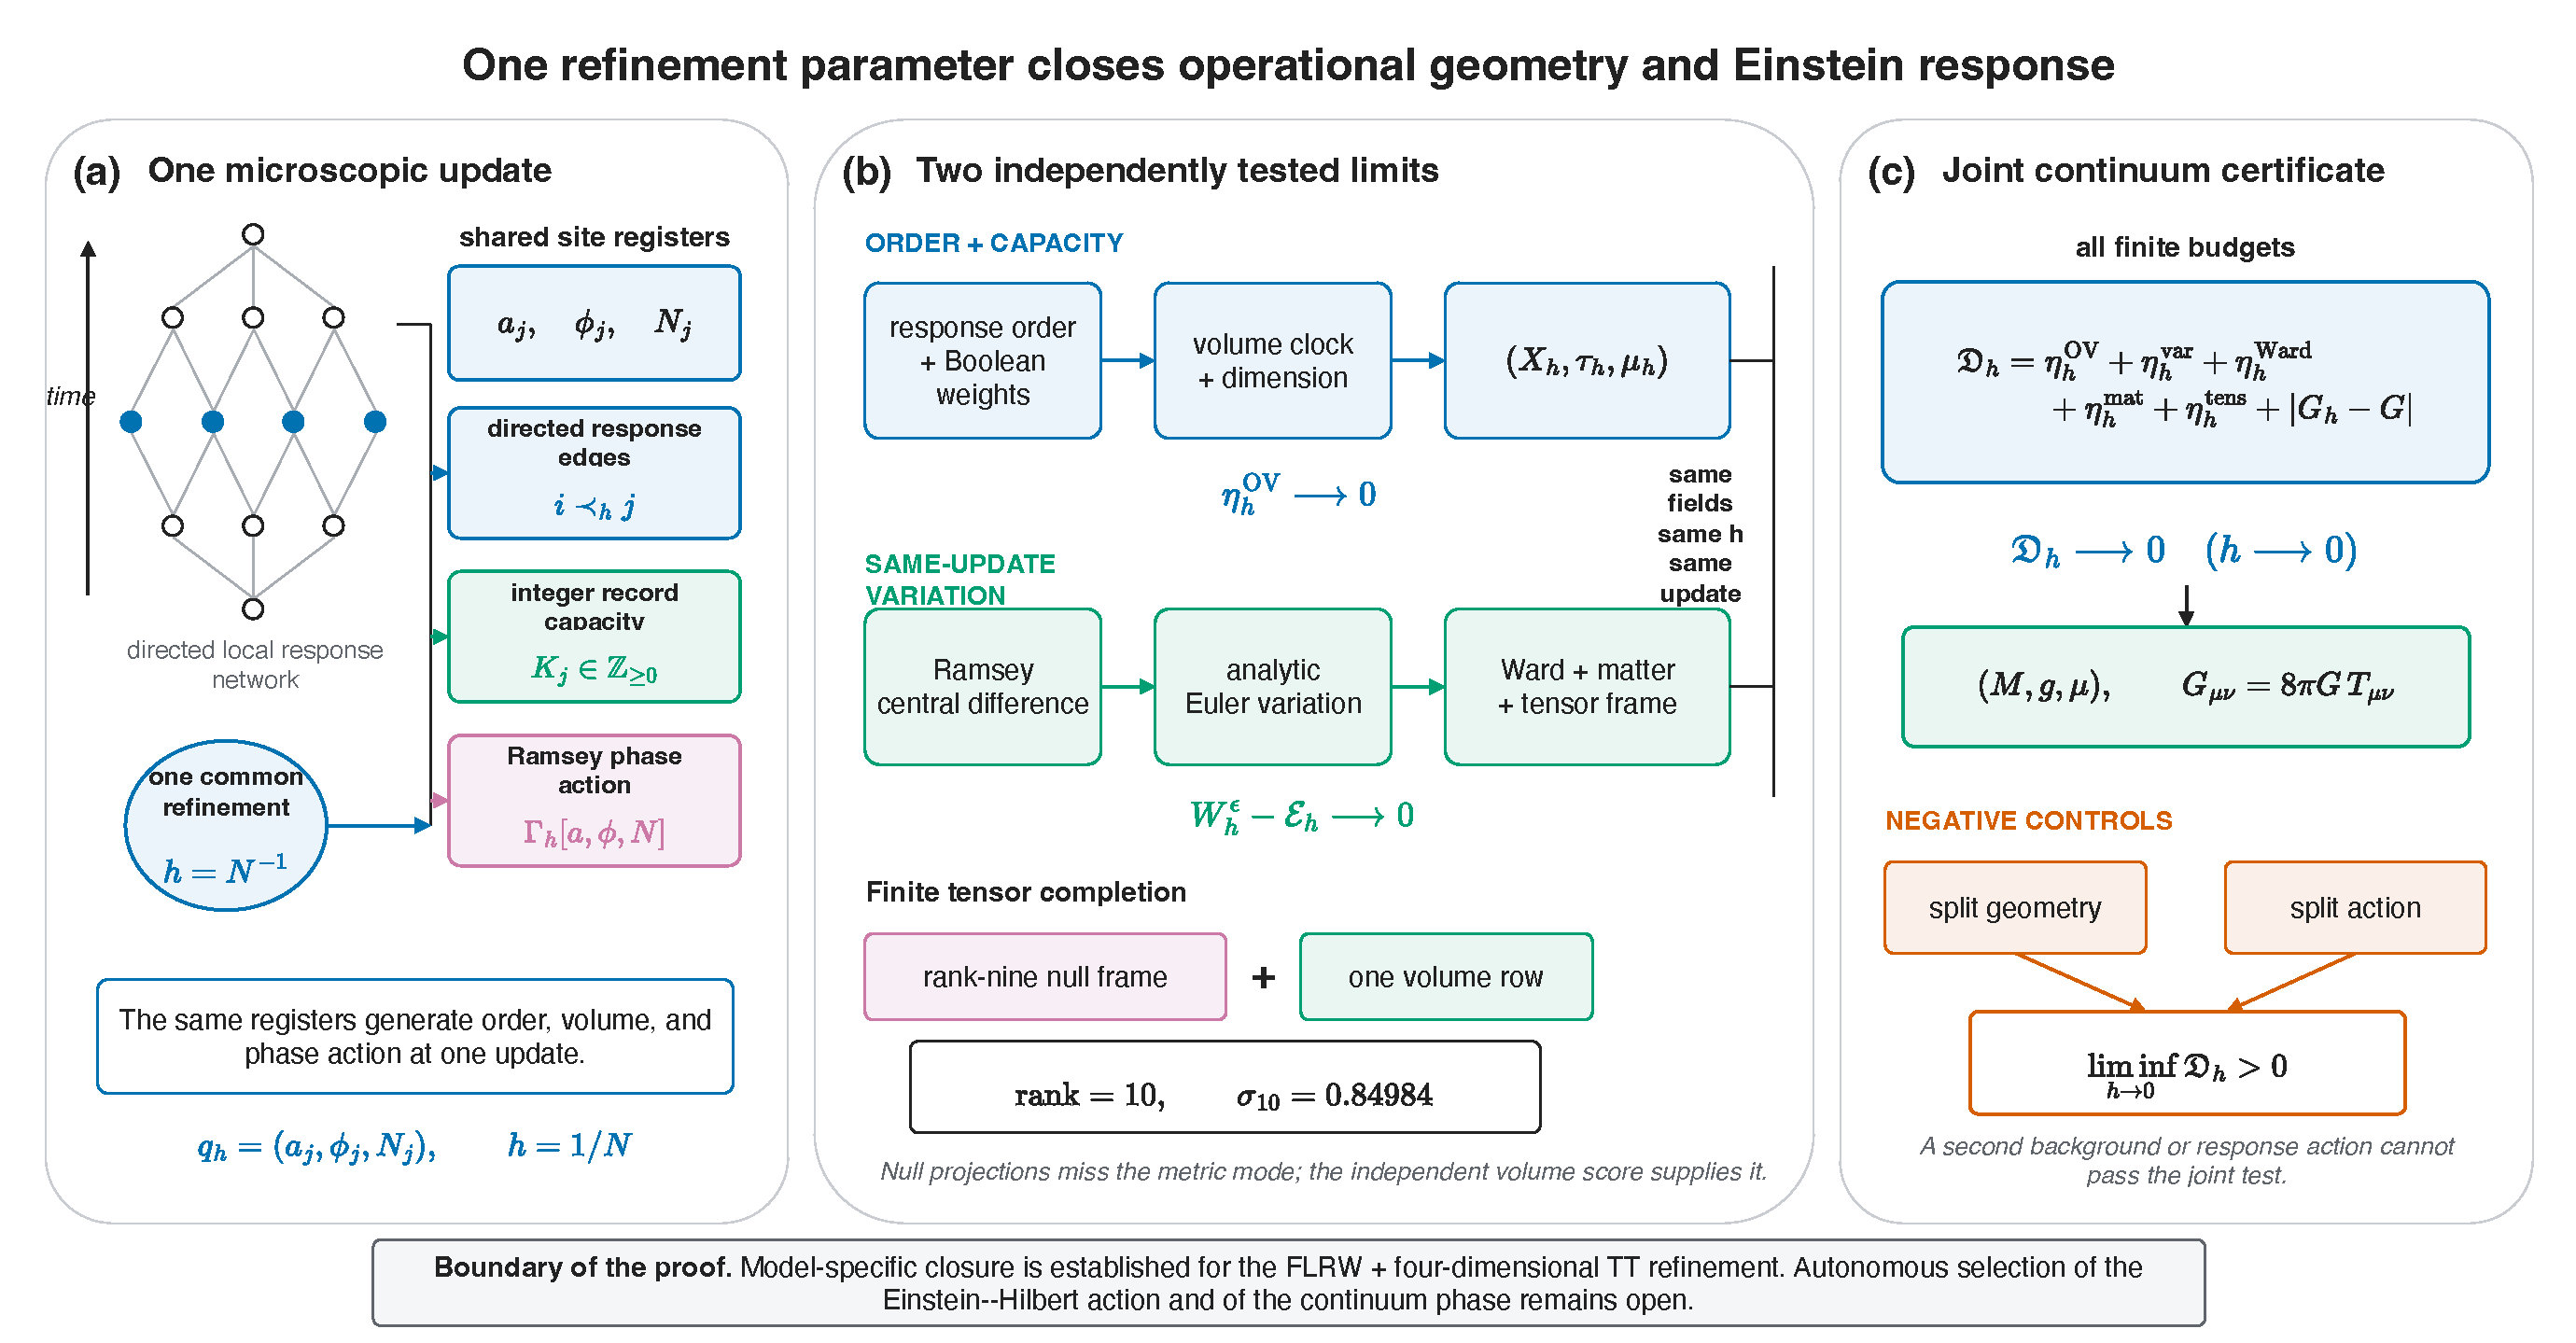
\includegraphics[width=0.97\linewidth]
 {figures/rqcp_qg_unified_continuum_v1.pdf}
 \caption{\textbf{Unified operational continuum limit.}
 Panel (a) records the common microscopic data: the same
 \(q_h=(a_j,\phi_j,N_j)\) and \(h=N^{-1}\) generate directed response
 records, integer Boolean capacities, and a Ramsey phase action.
 Panel (b) keeps geometry reconstruction and analytic variation independent;
 rank-nine null data plus one volume row determine all ten components of a
 symmetric four-tensor.  Panel (c) collects every finite defect before the
 limit is taken.  Split-geometry and split-action controls retain a nonzero
 floor.  The gray boundary box lists the inputs that the theorem does not
 select.  The figure is vector and its editable source is distributed with
 the companion manuscript.}
 \label{fig:unified-continuum-mechanism}
\end{figure}
\end{landscape}

\subsection{The joint finite certificate}

Let \(\eta_h^{\rm OV}\) bound the measured Lorentzian reconstruction error,
\(\eta_h^{\rm var}\) the error made by interchanging variation and
refinement, \(\eta_h^{\rm Ward}\) the finite Noether defect,
\(\eta_h^{\rm mat}\) the independently evaluated matter equation residual,
and \(\eta_h^{\rm tens}\) the error in completing the symmetric metric Euler
tensor from operational projections.  Let \(B_h\) be the compatible finite
divergence.  Taylor's formula applied to
Eq.~\eqref{eq:unified-ramsey-score} gives
\begin{equation}
 \|W_h^\varepsilon-{\cal E}_h\|_h
 \le\frac{\varepsilon^2}{6}M_{0,h},
 \qquad
 \|B_h(W_h^\varepsilon-{\cal E}_h)\|_h
 \le\varepsilon^2M_{1,h}.
 \label{eq:unified-central-difference}
\end{equation}
The second bound is imposed on the differentiated remainder field itself;
the cruder estimate \(\|B_h\|M_{0,h}\) can lose a power of \(h\).

At each event, contract a symmetric tensor with a finite set of normalized
null rows
\(A_\ell[X]=X_{\mu\nu}\ell^\mu\ell^\nu\).  These rows have rank at most nine
in four dimensions because they annihilate the metric direction.  Adding
one normalized volume row \(A_V[X]=g^{\mu\nu}X_{\mu\nu}\) gives a full frame
\(A_h\).  If
\(\sigma_{\min}(A_h)\ge\sigma_*>0\), then
\begin{equation}
 \|X\|_2\le\sigma_*^{-1}\|A_hX\|_2 .
 \label{eq:unified-frame-bound}
\end{equation}
The volume score is thus information-theoretically nonredundant; no further
null direction can replace it.

Define
\begin{align}
 {\mathfrak D}_h={}&
 \eta_h^{\rm OV}
 +\Delta_h^{\rm same}
 +\eta_h^{\rm var}
 +\frac{\varepsilon_h^2}{6}M_{0,h}
 +\varepsilon_h^2M_{1,h}\nonumber\\
 &+\eta_h^{\rm Ward}
 +\eta_h^{\rm mat}
 +\sigma_*^{-1}\eta_h^{\rm tens}
 +|G_h-G|.
 \label{eq:unified-certificate}
\end{align}
Every term is a finite-resolution quantity.  In particular, the Newton
coefficient is not hidden in the tensor norm: if it is supplied rather than
derived, the term \(|G_h-G|\) records that fact.

\begin{theorem}[Unified operational continuum limit]
\label{thm:unified-operational-continuum}
Let \(\{{\cal R}_h\}\) be a single-update refinement family on a compact
globally hyperbolic test region.  Suppose:
\begin{enumerate}[label=(U\arabic*)]
\item the order--volume reconstruction obeys
\(d_{\mathrm{mL}}[{\cal X}_h,({\cal M},\tau_g,\mu_g)]
\le\eta_h^{\rm OV}\to0\);
\item sampling and interpolation are stable and
\(\|{\cal I}_h{\cal E}_h-{\cal E}(g,\psi)\|_{H^{-1}}
\le\eta_h^{\rm var}\to0\);
\item Eq.~\eqref{eq:unified-central-difference} holds and
\(\varepsilon_h^2(M_{0,h}+M_{1,h})\to0\);
\item the null-plus-volume frame satisfies
\(\sigma_{\min}(A_h)\ge\sigma_*>0\); and
\item the Ward, matter, tensor, and coupling errors in
Eq.~\eqref{eq:unified-certificate} vanish.
\end{enumerate}
Then the operational geometry and response converge jointly:
\begin{align}
 d_{\mathrm{mL}}[{\cal X}_h,({\cal M},\tau_g,\mu_g)]
 &\le {\mathfrak D}_h,\label{eq:unified-geometry-limit}\\
 \|{\cal I}_hW_h^{\varepsilon_h}-{\cal E}(g,\psi)\|_{H^{-1}}
 &\le C_{\cal I}{\mathfrak D}_h .
 \label{eq:unified-dynamics-limit}
\end{align}
If a compactly convergent sequence also has vanishing operational score,
\(\|{\cal I}_hW_h^{\varepsilon_h}\|_{H^{-1}}\to0\), then
\({\cal E}(g,\psi)=0\) on the same metric--measure geometry selected by
Eq.~\eqref{eq:unified-geometry-limit}.  For the Einstein--matter action,
\begin{equation}
 G_{\mu\nu}[g]+\Lambda g_{\mu\nu}
 =8\pi G\,T_{\mu\nu}[g,\psi],
 \qquad {\cal E}_{\psi}(g,\psi)=0
 \label{eq:unified-einstein-limit}
\end{equation}
in the weak sense.
\end{theorem}

\begin{proof}
Insert \({\cal E}_h\) between the Ramsey score and the continuum Euler
covector.  Stable interpolation, the two estimates in
Eq.~\eqref{eq:unified-central-difference}, and variational consistency give
the projected response bound.  The rank-nine null frame reconstructs the
nonmetric tensor sector; Eq.~\eqref{eq:unified-frame-bound} and the volume
row add the missing metric component.  The Ward and matter terms control the
finite conservation and off-shell matter defects.  The order--volume term
fixes the continuum geometry, and
\(\Delta_h^{\rm same}\) prevents a second geometry from entering the phase
branch.  The triangle inequality yields
Eq.~\eqref{eq:unified-dynamics-limit}.  Passing to a compact limit of
vanishing operational scores gives
Eq.~\eqref{eq:unified-einstein-limit}.  No unproved interchange of
variation and limit occurs; its entire cost is \(\eta_h^{\rm var}\).
\end{proof}

\begin{corollary}[Split-limit rejection]
\label{cor:unified-split-rejection}
If \(\liminf_{h\to0}\Delta_h^{\rm same}>0\), or if the Ramsey branch uses
\(\Gamma_h+Q_h\) while the analytic branch varies \(\Gamma_h\) and
\(\liminf\|{\cal I}_hDQ_h\|>0\), then
\(\liminf_{h\to0}{\mathfrak D}_h>0\).
\end{corollary}

\subsection{Explicit FLRW--tensor realization}

The theorem is realized on
\begin{equation}
 {\cal M}=[1,2]\times\mathbb T^3,\qquad
 \mathrm ds^2=-\mathrm dt^2+a(t)^2\mathrm d\bm x^2 ,
 \label{eq:unified-flrw-metric}
\end{equation}
with \(8\pi G=1\) and
\begin{equation}
 a(t)=t^{1/3},\qquad
 \phi(t)=\sqrt{\frac23}\log t,\qquad
 N(t)=1 .
 \label{eq:unified-flrw-solution}
\end{equation}
For \(h=N^{-1}\), the same samples
\(q_h=(a_j,\phi_j,N_j)\) determine all three branches.  With
\(\eta(t)=\tfrac32t^{2/3}\), the response order is
\begin{equation}
 (j,\bm n)\prec_h(k,\bm m)
 \quad\Longleftrightarrow\quad
 j<k,\qquad
 h\,d_{\mathbb T^3}(\bm n,\bm m)
 <\eta(t_k)-\eta(t_j).
 \label{eq:unified-flrw-order}
\end{equation}
Each four-cell carries the Boolean capacity and weight
\begin{equation}
 C_j=\operatorname{round}\!\left[(N^3+1)a(t_{j+1/2})^3\right],
 \qquad
 w_j=h^4\frac{C_j}{N^3+1}.
 \label{eq:unified-capacity}
\end{equation}
The weighted counting measure converges to
\(a^3\,\mathrm dt\,\mathrm d^3x\).  Applying the intrinsic local
volume clock of Sec.~\ref{sec:generic-order-volume} on pieces of proper size
\(r_h\) gives
\begin{equation}
 |\widehat\tau_h-\tau_g|
 \le C\left(r_h^2+\frac{h}{r_h}+h^2+h^3\right).
 \label{eq:unified-order-volume-rate}
\end{equation}
The terms arise from small-diamond curvature, the lattice boundary shell,
midpoint quadrature, and capacity quantization.  Choosing
\(r_h=h^{1/3}\) gives the conservative complete clock rate
\(\eta_h^{\rm OV}=O(h^{2/3})\); the weak measure and local homogeneous metric
converge faster.

The phase branch uses the same samples in the midpoint
Einstein--massless-scalar functional
\begin{align}
 \Gamma_h[a,\phi,N]
 =\sum_{j=0}^{N-1}h\bigg[
 -\frac{3\bar a_j}{N_j}
  \left(\frac{a_{j+1}-a_j}{h}\right)^2
 +\frac{\bar a_j^3}{2N_j}
  \left(\frac{\phi_{j+1}-\phi_j}{h}\right)^2
 \bigg],
 \label{eq:unified-discrete-action}\\
 \bar a_j=\tfrac12(a_j+a_{j+1}).
 \nonumber
\end{align}
It generates the diagonal Ramsey phase and is varied independently to
obtain \({\cal E}_h\).  The variational, finite Ward, and scalar Euler
residuals converge at second order.  A periodic \(N^4\)
transverse-traceless sector supplies genuinely four-dimensional tensor
data.  Thirty rational null directions give rank nine; adding the volume
row gives rank ten with
\begin{equation}
 \sigma_{10}=0.8498365856 .
 \label{eq:unified-frame-sigma}
\end{equation}
The TT Ramsey--Euler defect is below \(3.01\times10^{-14}\), and the tensor
reconstruction error converges with fitted power \(1.951\).

\begin{figure}[htbp]
 \centering
 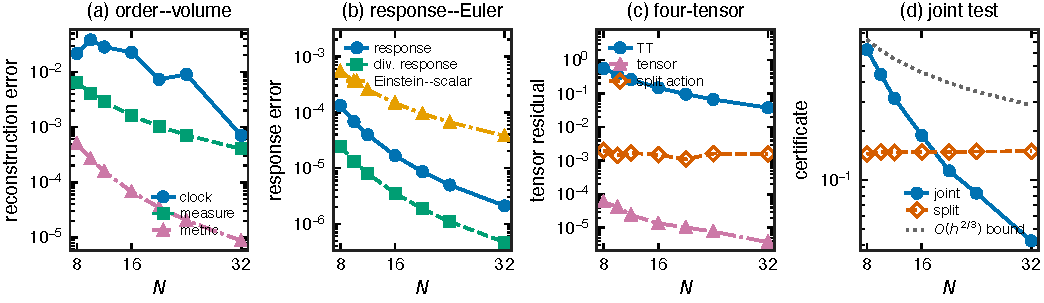
\includegraphics[width=\linewidth]
 {figures/rqcp_qg_unified_continuum_data_v1.pdf}
 \caption{\textbf{Deterministic synthetic refinement tests for the unified
 continuum certificate.}
 All panels use the common sizes \(N=8,10,12,16,20,24,32\).
 The order--volume observables, independent Ramsey/variation defects, and
 four-dimensional tensor residuals decrease under the same refinement.
 The complete certificate falls from \(0.630515\) to \(0.042254\), with
 fitted power \(1.949\) over the displayed sizes.  The gray
 \(O(h^{2/3})\) line is the conservative analytic envelope for the complete
 volume clock, not a fitted exponent.  Deliberately split geometry and
 action branches remain between \(0.1437\) and \(0.1498\).  These are
 reproducible synthetic calculations, not experimental data.}
 \label{fig:unified-continuum-data}
\end{figure}

The numerical archive contains 467 independent algebraic, refinement,
conditioning, split-control, and figure-data checks with no failed test.
The measured joint certificate decreases from \(0.630515\) at \(N=8\) to
\(0.042254\) at \(N=32\).  The split control remains between \(0.1437\) and
\(0.1498\), the minimum theorem-bound/actual-tensor-error ratio is \(1.7405\),
and the fitted powers of the Ward, Einstein--scalar, TT, tensor, and joint
errors are respectively \(1.898\), \(1.927\), \(1.945\), \(1.951\), and
\(1.949\).  These fitted powers diagnose this smooth family; the proved
order--volume statement remains the conservative
\(O(h^{2/3})\) estimate in
Eq.~\eqref{eq:unified-order-volume-rate}.

\subsection{Boundary of the result}

The model removes the possibility that the order--volume and
Einstein-response limits are mutually incompatible merely because they use
different discrete fields or different refinement maps.  It establishes a
nonempty, falsifiable realization in which one \(h\), one register family,
one capacity measure, and one phase action pass a common finite certificate.
It does \emph{not} remove the general assumptions \(A9V\) or \(A11\).
Specifically:
\begin{enumerate}
\item the four-dimensional manifold and \(\mathbb T^3\) topology are inputs;
\item the Einstein--Hilbert plus massless-scalar action is supplied, not
selected by a less structured microscopic channel;
\item the integer capacity unit and \(G_h=G\) are fixed microscopically;
\item the proof covers nonlinear homogeneous geometry and local
four-dimensional TT refinement, not arbitrary nonlinear inhomogeneous
spacetimes;
\item quantum fluctuations, renormalization, autonomous clock selection, and
a probability-law continuum limit remain open.
\end{enumerate}
The separate same-link construction in
Sec.~\ref{sec:same-link-induced-gravity} removes the supplied-curvature-action
input and controls large-\(N_s\) quantum fluctuations only for one
fixed-volume TT polarization at fixed microscopic spacing.  It does not
upgrade the present FLRW--Einstein--matter theorem to a general quantum
probability-law continuum limit.
The result is therefore a \emph{model-specific unified continuum closure}.
The general target remains one autonomous local quantum dynamics that
selects its manifoldlike phase, capacity-density law, gravitational action,
and regulator-independent Newton coefficient.
